% !TeX program = xelatex
%==============================================================
%  Python金融数据分析 · 第10章 统计学与投资组合优化
%  基于《Python金融大数据分析（第2版）》第13章 13.1--13.2 节
%  配套课堂代码：notebooks/10_Statistics_Portfolio_Optimization.ipynb
%==============================================================
\documentclass[9pt]{ctexbeamer}

\usepackage{style/shubeamer}
\usepackage{amsmath,amsfonts,amssymb,bm}
\usepackage{graphicx,hyperref,url}
\usepackage{subcaption}
\usepackage{booktabs}
\usepackage[super,square]{natbib}
\usepackage{wrapfig}
\usepackage{calligra}

\setmainfont{CMU Serif}
\setsansfont{CMU Sans Serif}

\definecolor{nvidia}{RGB}{102,156,28}
\definecolor{red}{RGB}{184,13,73}
\definecolor{orange}{RGB}{242,151,36}
\definecolor{darkteal}{RGB}{43,106,108}
\definecolor{darkblue}{RGB}{4,37,58}

\AtBeginSection[]
{
  \begin{frame}<beamer>
    \frametitle{\textbf{目录}}
    \textbf{\tableofcontents[currentsection]}
  \end{frame}
}

\graphicspath{{figures/}}

\AtBeginDocument{%
  \title[Python金融数据分析 · 第10章]{\fontsize{16pt}{22pt}\selectfont {Python金融数据分析}}
  \subtitle{\fontsize{9pt}{14pt}\selectfont \textit{第10章\quad 统计学与投资组合优化}}
  \author[王伟冠, 吕文俊]{%
    \begin{tabular}{ll}%
      主讲人： & 王伟冠, 吕文俊\tabularnewline%
      院\quad 系： & 经济学院金融系\tabularnewline
    \end{tabular}
  }
  \institute[SHU]{上海大学}
  \date[\today]{\today}}

\input{style/macros.tex}

\begin{document}

\begin{frame}
  \titlepage
\end{frame}

\section*{目录}
\begin{frame}
  \frametitle{\textbf{目录}}
  \textbf{\tableofcontents}
\end{frame}

%==============================================================
\section{正态性检验}
%==============================================================

\begin{frame}{本章学习目标}
  \begin{itemize}
    \item 理解为什么\textbf{收益率的正态性}是许多金融模型的出发点。
    \item 会用直方图、QQ 图、偏度/峰度和 $p$ 值检验收益率的正态性。
    \item 会把日度价格转换为\textbf{对数收益率}，并解释现实数据中的肥尾现象。
    \item 会在仅做多约束下，用 Python 构造\textbf{随机组合、最优组合和有效边界}。
  \end{itemize}
  \begin{block}{本章主线}
    先问：\alert{收益率的分布像正态分布吗？}\quad
    再问：如果用均值和协方差描述风险收益，\alert{怎样配置一篮子资产？}
  \end{block}
\end{frame}

\begin{frame}{正态性是均值--方差分析的共同语言}
  \begin{columns}[T,totalwidth=\textwidth]
    \begin{column}{0.48\textwidth}
      \textbf{若收益近似正态分布}
      \begin{itemize}
        \item 均值描述收益的中心；方差/波动率描述风险。
        \item 投资者的选择可归结为：\alert{在收益和风险之间权衡}。
        \item 均值--方差理论、CAPM 等模型更容易成立。
      \end{itemize}
    \end{column}
    \begin{column}{0.48\textwidth}
      \textbf{但真实市场往往不同}
      \begin{itemize}
        \item 极端涨跌比正态分布预言得更多，称为\alert{肥尾}。
        \item 可能存在偏度、波动聚集和结构变化。
        \item 所以检验不是为了证明模型“正确”，而是了解模型的\textbf{适用边界}。
      \end{itemize}
    \end{column}
  \end{columns}
  \vspace{0.5em}
  \begin{center}
    本节改编自教材第13.1节\citep{hilpisch2018python}。
  \end{center}
\end{frame}

\begin{frame}[fragile]{基准案例：几何布朗运动的对数收益}
  \begin{itemize}
    \item 几何布朗运动（GBM）是金融建模的常见基准；其单期\textbf{对数收益}服从正态分布：
  \end{itemize}
  \begin{equation*}
    \ln\frac{S_t}{S_{t-\Delta t}}
    = \left(r-\frac{1}{2}\sigma^2\right)\Delta t
      +\sigma\sqrt{\Delta t}\,z_t,\qquad z_t\sim N(0,1)
  \end{equation*}
\begin{lstlisting}
def gbm_paths(S0=100, r=0.05, sigma=0.20, steps=50):
    dt = 1 / steps
    shocks = rng.standard_normal((steps, paths))
    # 每一步将随机冲击乘到当前价格上
\end{lstlisting}
  \begin{alertblock}{注意}
    \textbf{价格}呈对数正态，而不是正态；检验对象通常是\alert{收益率}或\alert{对数收益率}。
  \end{alertblock}
\end{frame}

\begin{frame}{模拟基准：直方图与理论密度几乎重合}
  \begin{center}
    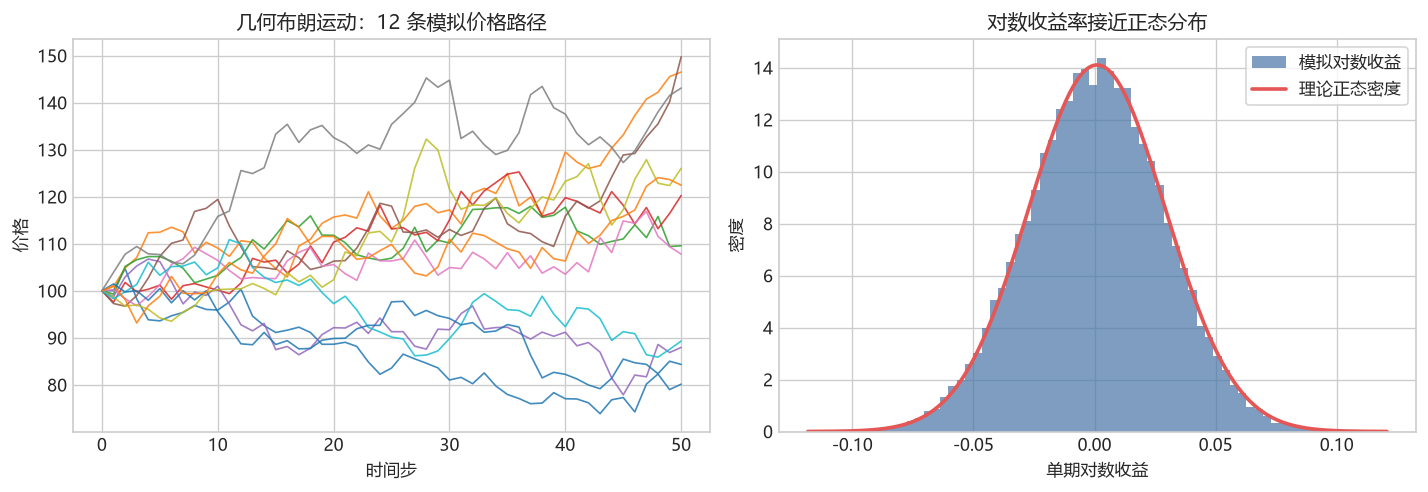
\includegraphics[width=0.92\textwidth]{ch10_gbm_normality}
  \end{center}
  \begin{itemize}
    \item 25{,}000 条 GBM 路径的抽样对数收益与理论正态密度吻合。
    \item 本次运行中，综合正态性检验的 $p=0.0995>0.05$：\textbf{不能拒绝}正态性假设。
  \end{itemize}
\end{frame}

\begin{frame}{四种工具：图形检验与统计检验互相补充}
  \begin{columns}[T,totalwidth=\textwidth]
    \begin{column}{0.48\textwidth}
      \begin{block}{图形工具：先看形状}
        \begin{itemize}
          \item \textbf{直方图 + 正态密度}：看中心、尾部和不对称性。
          \item \textbf{QQ 图}：样本分位数若贴近直线，则更接近正态；两端偏离提示肥尾。
        \end{itemize}
      \end{block}
    \end{column}
    \begin{column}{0.48\textwidth}
      \begin{block}{统计工具：量化偏离}
        \begin{itemize}
          \item 偏度：正态分布的理论值为 0。
          \item 超额峰度：正态分布的理论值为 0；正值通常提示肥尾。
          \item \texttt{scipy.stats.normaltest}：原假设为“样本来自正态分布”。
        \end{itemize}
      \end{block}
    \end{column}
  \end{columns}
  \begin{exampleblock}{怎样读 $p$ 值？}
    在 5\% 显著性水平，$p<0.05$ 时拒绝正态性；$p\geq0.05$ 只意味着\textbf{没有足够证据拒绝}，不是“证明正态”。
  \end{exampleblock}
\end{frame}

\begin{frame}{真实数据：四个资产的尾部显著偏离正态}
  \begin{center}
    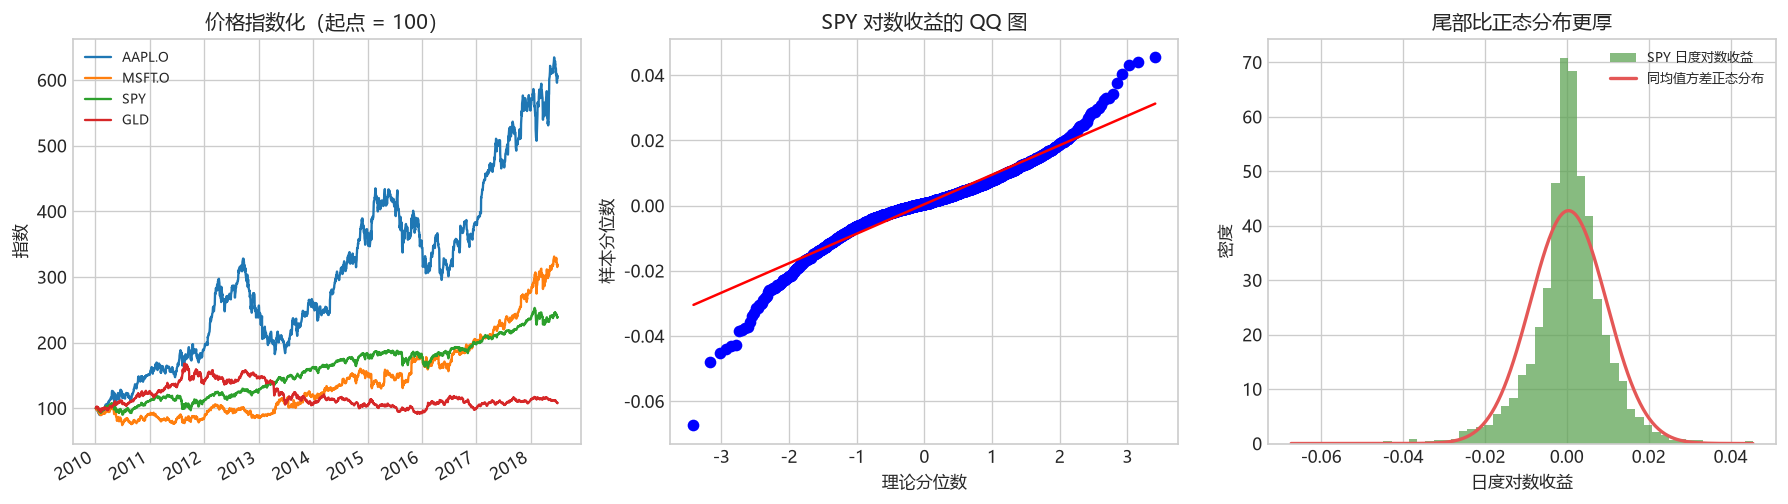
\includegraphics[width=0.97\textwidth]{ch10_real_data_normality}
  \end{center}
  \begin{itemize}
    \item 数据为 2010-01-04 至 2018-06-29 的 2{,}137 个日度对数收益观测值。
    \item AAPL、MSFT、SPY 和 GLD 的正态性检验 $p$ 值均小于 0.0001；SPY 的 QQ 图两端尤其明显地偏离直线。
  \end{itemize}
\end{frame}

\begin{frame}{正态性检验的结论：模型是近似，不是承诺}
  \begin{itemize}
    \item 用正态分布建模可带来清晰、可计算的基准；GBM 是一个好例子。
    \item 真实收益率往往有\alert{肥尾和负偏}：低估尾部风险会使风险管理过于乐观。
    \item 均值--方差优化仍然有教学和实践价值，但必须承认它高度依赖\textbf{收益与协方差估计}。
  \end{itemize}
  \begin{block}{过渡问题}
    已经有了多种资产的历史收益率：如何把它们组合起来，既追求收益，又控制波动？
  \end{block}
\end{frame}

%==============================================================
\section{投资组合优化}
%==============================================================

\begin{frame}{本节数据：四种资产与两个统计输入}
  \begin{columns}[T,totalwidth=\textwidth]
    \begin{column}{0.40\textwidth}
      \begin{table}
        \centering
        \caption{本章组合资产}
        \begin{tabular}{ll}
          \toprule
          代码 & 含义 \\
          \midrule
          AAPL.O & Apple 股票 \\
          MSFT.O & Microsoft 股票 \\
          SPY & S\&P 500 ETF \\
          GLD & 黄金 ETF \\
          \bottomrule
        \end{tabular}
      \end{table}
    \end{column}
    \begin{column}{0.55\textwidth}
      \begin{block}{均值--方差优化只需要两类输入}
        \begin{itemize}
          \item 预期收益向量 $\bm{\mu}$：本例用历史日均对数收益乘以 252 年化。
          \item 协方差矩阵 $\bm{\Sigma}$：衡量单个资产风险及资产之间的共同波动。
        \end{itemize}
      \end{block}
      \begin{itemize}
        \item 本次样本的年化平均收益：AAPL 21.24\%、MSFT 13.66\%、SPY 10.29\%、GLD 0.91\%。
        \item \alert{协方差}是分散化的关键：低相关资产可降低组合波动。
      \end{itemize}
    \end{column}
  \end{columns}
\end{frame}

\begin{frame}{基本理论：权重把单个资产变成组合}
  \begin{itemize}
    \item 用权重向量 $\bm{w}=(w_1,\dots,w_n)^\mathsf{T}$ 描述配置；本节只允许多头：
  \end{itemize}
  \begin{equation*}
    \sum_{i=1}^n w_i=1,\qquad 0\leq w_i\leq 1
  \end{equation*}
  \begin{columns}[T,totalwidth=\textwidth]
    \begin{column}{0.48\textwidth}
      \begin{block}{预期组合收益}
        \begin{equation*}
          \mu_p=\bm{w}^\mathsf{T}\bm{\mu}
        \end{equation*}
        权重越高的资产，对期望收益的影响越大。
      \end{block}
    \end{column}
    \begin{column}{0.48\textwidth}
      \begin{block}{组合波动率}
        \begin{equation*}
          \sigma_p=\sqrt{\bm{w}^\mathsf{T}\bm{\Sigma}\bm{w}}
        \end{equation*}
        不只看单个资产波动率，还要看\alert{协方差}。
      \end{block}
    \end{column}
  \end{columns}
  \vspace{0.5em}
  \begin{center}
    $\bm{w}^\mathsf{T}\bm{\Sigma}\bm{w}$ 正是 NumPy 矩阵乘法的直接翻译。\citep{hilpisch2018python}
  \end{center}
\end{frame}

\begin{frame}[fragile]{随机权重：先画出可能的风险--收益空间}
\begin{lstlisting}
annual_returns = log_returns.mean() * 252
annual_covariance = log_returns.cov() * 252

weights = rng.dirichlet(np.ones(4), size=5000)
port_ret = weights @ annual_returns.to_numpy()
port_vol = np.sqrt(np.einsum('ij,jk,ik->i',
                             weights, annual_covariance, weights))
\end{lstlisting}
  \begin{itemize}
    \item \texttt{dirichlet} 每次生成一组非负且和为 1 的权重，正好满足长仓预算约束。
    \item 每个点是一组配置；横轴是年化波动率，纵轴是年化预期收益。
    \item 颜色使用夏普比率：$\mathrm{SR}=(\mu_p-r_f)/\sigma_p$，本例取 $r_f=1\%$。
  \end{itemize}
\end{frame}

\begin{frame}{随机组合不是答案，却揭示了可选空间}
  \begin{center}
    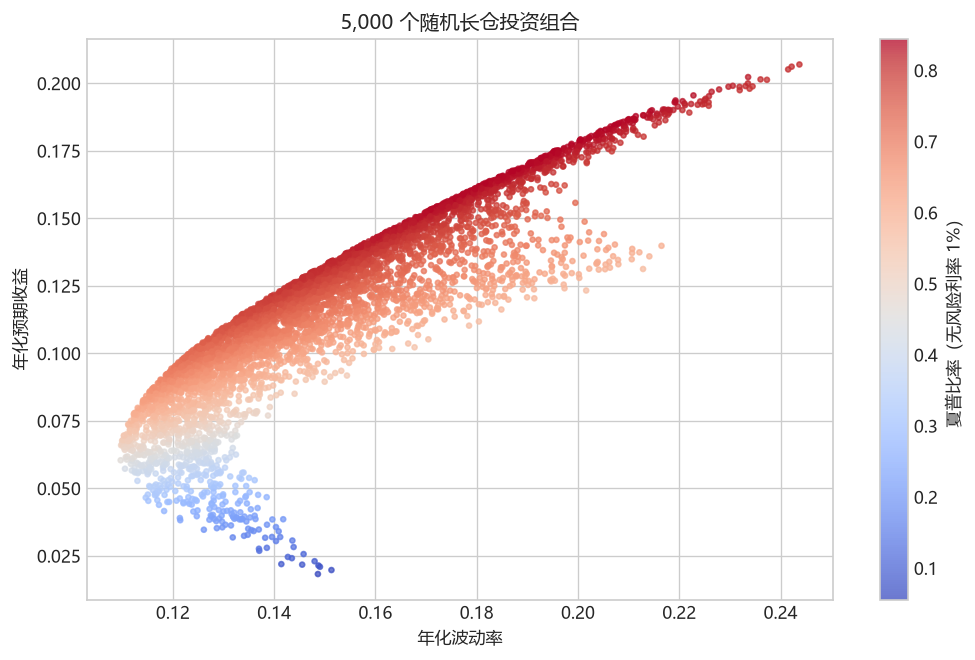
\includegraphics[width=0.78\textwidth]{ch10_random_portfolios}
  \end{center}
  \begin{itemize}
    \item 给定相近的风险，仍可能有收益明显不同的配置；大多数随机点并不有效。
    \item 图的上边界附近，是“在相同风险下更高收益”或“相同收益下更低风险”的候选组合。
  \end{itemize}
\end{frame}

\begin{frame}{优化问题：把“更好”写成目标和约束}
  \begin{columns}[T,totalwidth=\textwidth]
    \begin{column}{0.48\textwidth}
      \begin{block}{最大夏普比率}
        \begin{equation*}
          \max_{\bm{w}}\ \frac{\mu_p-r_f}{\sigma_p}
        \end{equation*}
        寻找每单位风险带来最高超额收益的组合。
      \end{block}
    \end{column}
    \begin{column}{0.48\textwidth}
      \begin{block}{全局最小方差}
        \begin{equation*}
          \min_{\bm{w}}\ \sigma_p
        \end{equation*}
        在给定可投资资产中寻找波动率最低的组合。
      \end{block}
    \end{column}
  \end{columns}
  \begin{alertblock}{两条约束必须同时交给优化器}
    预算约束：$\sum_i w_i=1$；长仓边界：$0\leq w_i\leq 1$。不写约束，答案可能隐含借贷或卖空。
  \end{alertblock}
\end{frame}

\begin{frame}[fragile]{用 SciPy 的 SLSQP 求解受约束问题}
\begin{lstlisting}
bounds = tuple((0.0, 1.0) for _ in ASSETS)
budget = {'type': 'eq', 'fun': lambda w: w.sum() - 1}

max_sharpe = optimize.minimize(negative_sharpe_ratio,
    equal_weights, method='SLSQP', bounds=bounds,
    constraints=budget)
min_variance = optimize.minimize(portfolio_volatility,
    equal_weights, method='SLSQP', bounds=bounds,
    constraints=budget)
\end{lstlisting}
  \begin{itemize}
    \item 两次优化共享相同的约束，只改变目标函数。
    \item 一定检查 \texttt{result.success}，并验证权重之和、边界和目标改进。
    \item 优化得到的是\alert{样本内最优}；输入估计变化时，权重也可能显著改变。
  \end{itemize}
\end{frame}

\begin{frame}{本次样本中，两种最优目标给出截然不同的配置}
  \begin{center}
    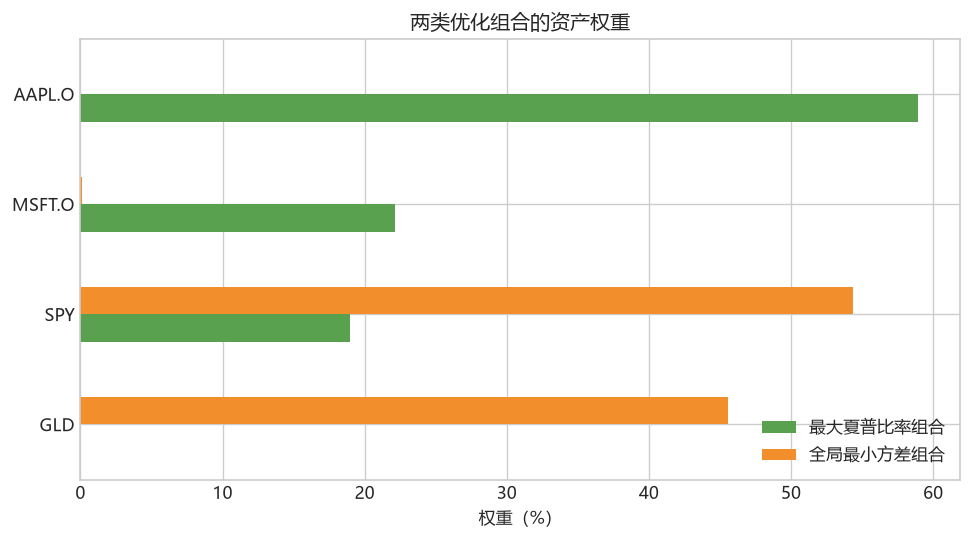
\includegraphics[width=0.82\textwidth]{ch10_optimized_weights}
  \end{center}
  \begin{itemize}
    \item 最大夏普比率：AAPL 58.9\%、MSFT 22.1\%、SPY 19.0\%；年化收益 17.49\%，波动率 19.52\%，夏普比率 0.845。
    \item 全局最小方差：SPY 54.3\%、GLD 45.6\%；年化收益 6.02\%，波动率 10.94\%。
  \end{itemize}
\end{frame}

\begin{frame}{有效边界：每一个目标收益对应最低可得风险}
  \begin{itemize}
    \item 固定目标收益 $\mu_p=\mu^*$，在预算约束和长仓边界下\textbf{最小化波动率}；重复求解即可追踪有效边界。
    \item 蓝线以下的随机点被边界支配；加入 $r_f=1\%$ 的无风险资产后，从 $(0,r_f)$ 作切线得到\alert{资本市场线}和切点组合。
  \end{itemize}
  \begin{center}
    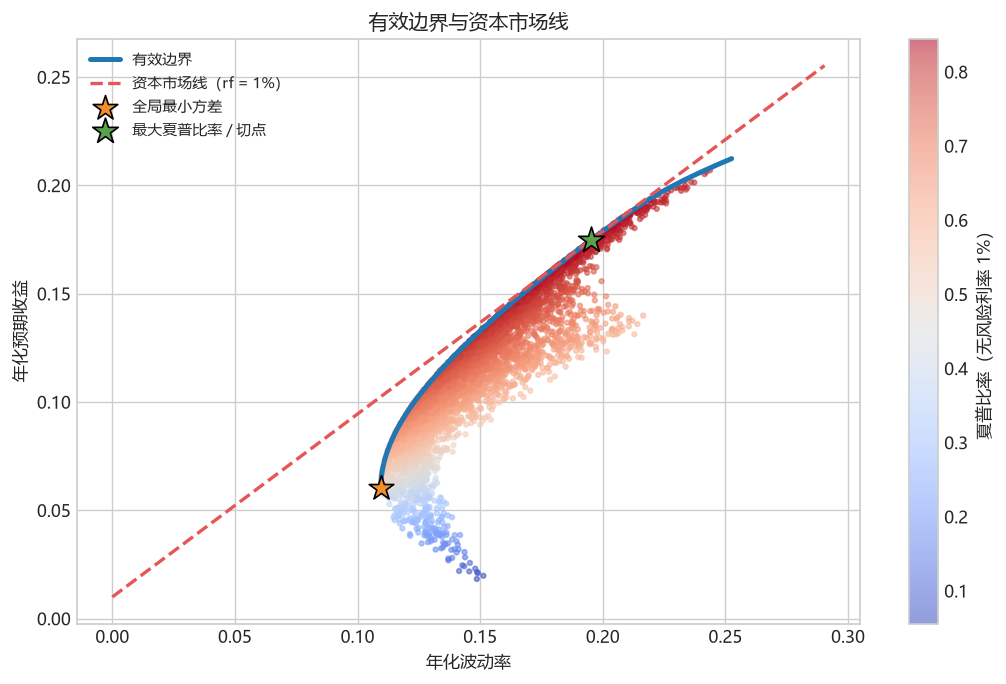
\includegraphics[width=0.72\textwidth]{ch10_efficient_frontier_cml}
  \end{center}
\end{frame}

\begin{frame}{如何把优化结果用于判断，而不是机械下单}
  \begin{itemize}
    \item \textbf{估计误差}：样本平均收益最不稳定；很小的输入变化可能导致很大的权重变化。
    \item \textbf{模型约束}：本例不允许卖空，也没有交易成本、税费、流动性和仓位上限。
    \item \textbf{样本外检验}：今天在样本内“最优”的权重，不保证明天仍然最优。
    \item \textbf{实务改进}：使用滚动窗口、收缩协方差、权重上限、再平衡成本和压力测试。
  \end{itemize}
  \begin{alertblock}{课程立场}
    均值--方差优化提供一套清晰的\textbf{决策语言}，而不是一台自动产生投资建议的机器。
  \end{alertblock}
\end{frame}

%==============================================================
\section{小结与练习}
%==============================================================

\begin{frame}{本章小结}
  \begin{itemize}
    \item \textbf{正态性检验}：直方图、QQ 图、偏度、峰度和 $p$ 值从不同角度检查分布；真实金融收益常有肥尾。
    \item \textbf{组合度量}：$\mu_p=\bm{w}^\mathsf{T}\bm{\mu}$，$\sigma_p=\sqrt{\bm{w}^\mathsf{T}\bm{\Sigma}\bm{w}}$；协方差决定分散化效果。
    \item \textbf{优化目标}：最大夏普比率追求风险调整后收益；最小方差追求最低组合波动；两者都要写清约束。
    \item \textbf{有效边界与资本市场线}：前者给出高风险资产的最优集合，后者将无风险资产纳入风险--收益选择。
  \end{itemize}
\end{frame}

\begin{frame}{课后任务与下章预告}
  \begin{block}{课后任务}
    \begin{enumerate}
      \item 在 notebook 中把无风险利率依次设为 0\%、2\%、3\%，比较资本市场线与最大夏普比率组合。
      \item 只选 SPY 与 GLD，画出两资产的所有长仓组合；解释它为何呈弯曲形状。
      \item 用 2010--2015 年估计参数、2016--2018 年评估表现；比较等权重与样本内最优组合。
    \end{enumerate}
  \end{block}
  \begin{exampleblock}{下章预告}
    组合优化依赖数值计算。下一章将讨论如何让 Python 代码跑得更快，并科学地度量性能。
  \end{exampleblock}
  \begin{center}
    配套代码：\texttt{10\_Statistics\_Portfolio\_Optimization.ipynb}
  \end{center}
\end{frame}

\appendix

\begin{frame}[allowframebreaks]{参考文献}
  \bibliographystyle{style/gbt7714-2005}
  \bibliography{reference.bib}
\end{frame}

\begin{frame}
  \begin{center}
    {\Huge\calligra Thanks for your attention!}
    \vspace{1cm}

    {\Huge Q \& A}
  \end{center}
\end{frame}

\end{document}
